
%(BEGIN_QUESTION)
% Copyright 2008, Tony R. Kuphaldt, released under the Creative Commons Attribution License (v 1.0)
% This means you may do almost anything with this work of mine, so long as you give me proper credit

Graph the output of this proportional-only controller, assuming a proportional band of 50\%, a bias value of 30\%, and a control action that is reverse-acting:

$$\includegraphics[width=15.5cm]{i03273x01.eps}$$

A direct method of solving for the output graph is to re-calculate the output value using the proportional controller equation ($m = K_p e + b$), at every point where there is a unique PV and/or SP value.  For example, you could use the equation to calculate the output value at PV=30\%, PV=20\%, and PV=25\%.  This involves repeated calculations, which may be tedious for a complex graph.  

As an aid to doing these repeated calculations, try setting up a computer spreadsheet (e.g. Microsoft Excel) to evaluate the proportional control equation for you, and then see if you can configure the spreadsheet to produce a graph of the same PV, SP, and Output trends as well!

\vskip 20pt \vbox{\hrule \hbox{\strut \vrule{} {\bf Suggestions for Socratic discussion} \vrule} \hrule}

\begin{itemize}
\item{} How would the output signal trend be altered if the {\it proportional band} of this controller were increased?
\item{} How would the output signal trend be altered if the {\it bias} of this controller were increased?
\item{} How would the output signal trend be altered if the {\it action} of this controller were switched from reverse to direct?
\end{itemize}

\underbar{file i03273}
%(END_QUESTION)





%(BEGIN_ANSWER)

$$\includegraphics[width=15.5cm]{i03273x02.eps}$$

%(END_ANSWER)





%(BEGIN_NOTES)

$$m = 2(\hbox{SP} - \hbox{PV}) + 30$$

% No blank lines allowed between lines of an \halign structure!
% I use comments (%) instead, so that TeX doesn't choke.

$$\vbox{\offinterlineskip
\halign{\strut
\vrule \quad\hfil # \ \hfil & 
\vrule \quad\hfil # \ \hfil & 
\vrule \quad\hfil # \ \hfil \vrule \cr
\noalign{\hrule}
%
% First row
{\bf PV} & {\bf SP} & {\bf Output} \cr
%
\noalign{\hrule}
%
% Another row
30\% & 40\% & 50\% \cr
%
\noalign{\hrule}
%
% Another row
20\% & 40\% & 70\% \cr
%
\noalign{\hrule}
%
% Another row
25\% & 40\% & 60\% \cr
%
\noalign{\hrule}
} % End of \halign 
}$$ % End of \vbox


%INDEX% Control, proportional: graphing controller response

%(END_NOTES)


